%%%%%%%% ICML 2025 EXAMPLE LATEX SUBMISSION FILE %%%%%%%%%%%%%%%%%

\documentclass{article}

% Recommended, but optional, packages for figures and better typesetting:
\usepackage{microtype}
\usepackage{graphicx}
\usepackage{subfigure}
\usepackage{booktabs} % for professional tables

% hyperref makes hyperlinks in the resulting PDF.
% If your build breaks (sometimes temporarily if a hyperlink spans a page)
% please comment out the following usepackage line and replace
% \usepackage{icml2025} with \usepackage[nohyperref]{icml2025} above.
\usepackage{hyperref}

% Attempt to make hyperref and algorithmic work together better:
\newcommand{\theHalgorithm}{\arabic{algorithm}}

% Use the following line for the initial blind version submitted for review:
% \usepackage{icml2025}

% If accepted, instead use the following line for the camera-ready submission:
\usepackage[accepted]{icml2025}

% For theorems and such
\usepackage{amsmath}
\usepackage{amssymb}
\usepackage{mathtools}
\usepackage{amsthm}

% % For code
% \usepackage{listings}
% \usepackage[frozencache,cachedir=.]{minted}

% if you use cleveref..
\usepackage[capitalize,noabbrev]{cleveref}

%%%%%%%%%%%%%%%%%%%%%%%%%%%%%%%%
% THEOREMS
%%%%%%%%%%%%%%%%%%%%%%%%%%%%%%%%
\theoremstyle{plain}
\newtheorem{theorem}{Theorem}[section]
\newtheorem{proposition}[theorem]{Proposition}
\newtheorem{lemma}[theorem]{Lemma}
\newtheorem{corollary}[theorem]{Corollary}
\theoremstyle{definition}
\newtheorem{definition}[theorem]{Definition}
\newtheorem{assumption}[theorem]{Assumption}
\theoremstyle{remark}
\newtheorem{remark}[theorem]{Remark}

% Todonotes is useful during development; simply uncomment the next line
%    and comment out the line below the next line to turn off comments
%\usepackage[disable,textsize=tiny]{todonotes}
% \usepackage[textsize=tiny]{todonotes}


% The \icmltitle you define below is probably too long as a header.
% Therefore, a short form for the running title is supplied here:
\icmltitlerunning{Re-Examine Hybrid State-Space and Self-Attention for In-Context Learning}

\begin{document}

\twocolumn[
\icmltitle{Re-Examine Hybrid State-Space and Self-Attention for In-Context Learning}

% It is OKAY to include author information, even for blind
% submissions: the style file will automatically remove it for you
% unless you've provided the [accepted] option to the icml2025
% package.

% List of affiliations: The first argument should be a (short)
% identifier you will use later to specify author affiliations
% Academic affiliations should list Department, University, City, Region, Country
% Industry affiliations should list Company, City, Region, Country

% You can specify symbols, otherwise they are numbered in order.
% Ideally, you should not use this facility. Affiliations will be numbered
% in order of appearance and this is the preferred way.
\icmlsetsymbol{equal}{*}

\begin{icmlauthorlist}
\icmlauthor{Jingze Shi}{equal,IR}
\icmlauthor{Bingheng Wu}{equal,IR}
\end{icmlauthorlist}

\icmlaffiliation{IR}{Independent Researcher}


\icmlcorrespondingauthor{Jingze Shi}{losercheems@gmail.com}
\icmlcorrespondingauthor{Bingheng Wu}{wubingheng52136@gmail.com}

% You may provide any keywords that you
% find helpful for describing your paper; these are used to populate
% the "keywords" metadata in the PDF but will not be shown in the document
\icmlkeywords{Machine Learning, ICML}

\vskip 0.3in
]



\begin{abstract}
% 最近的研究表明, 将状态空间算法驱动的 Mamba 与自注意力算法驱动的 Transformer 相结合, 在大多数语言建模任务上的表现超越了单独使用 Mamba 或 Transformer. 
% 但是, 目前主流的混合建模架构模型在情景学习任务上的表现并不理想, 我们重新审视了这两种算法的优势和劣势, 从原理出发对这种混合建模的结构重新设计. 
% 最终, 重新设计的架构, 在标准短文本任务中提升了 1.3 \% 效果, 在自然长文本任务中提升了 20.86 \% 效果, 在合成长文本任务中提升了 27.06 \% 效果.
Recent research has shown that combining the state-space algorithm-driven Mamba with the self-attention algorithm-driven Transformer outperforms using Mamba or Transformer alone in most language modeling tasks. However, the performance of the mainstream hybrid modeling architecture models in in-context learning tasks is not ideal. We re-examine the advantages and disadvantages of these two algorithms and redesign the structure of this hybrid modeling from the principle. The finally redesigned architecture improves the performance by 1.3\% in standard short text tasks, 20.86\% in natural long text tasks, and 27.06\% in synthetic long text tasks.
\end{abstract}

\section{Introduction}
\label{submission}
% Transformers~\cite{transformer2017} 架构的自注意力算法能够直接捕捉序列中任意两个元素间的关系, 有效处理长距离依赖问题. 但是却受到二次复杂度的限制.
% Mamba~\cite{gu2023mamba} 架构的状态空间算法能够在训练期间实现序列长度的线性缩放, 并在生成期间保持恒定的状态大小, 但是却在捕捉长距离依赖问题上导致偏差.
% 混合建模架构模型, 例如 Wonderful Matrices~\cite{shi2024wonderfulmatrices}, Jamba~\cite{lieber2024jamba}, 等等, 使用状态空间和自注意力进行混合建模, 使模型具备与 Mamba 类似的效率和与 Transformer 类似的效果. 然而, 这些模型在情景学习任务上的表现却与原始的 Transformer 相比, 仍然有不小的差距.
The self-attention algorithm of the Transformers~\cite{wolf-etal-2020-transformers} architecture can directly capture the relationship between any two elements in a sequence, effectively handle long-distance dependencies. However, it is limited by quadratic complexity. The state-space algorithm of the Mamba~\cite{gu2023mamba} architecture can achieve linear scaling of sequence length during training and maintain a constant state size during generation, but it leads to bias in capturing long-distance dependencies. Hybrid modeling architecture models, such as Wonderful Matrices~\cite{shi2024wonderfulmatrices}, Jamba~\cite{lieber2024jamba}, etc., use state-space and self-attention for hybrid modeling, making the model have efficiency similar to The Mamba and effect similar to The Transformer. However, these models still have a significant gap in performance in in-context learning tasks compared to the original Transformer.

% 我们提出了 Self-Attention before LM-Head~\ref{fig:architecture}, 这是对现有的混合堆叠架构模型的一种简单改变, 将状态空间和自注意力修改为使用相同的位置编码, 并在 LM-Head 预测概率分布之前使用自注意力和前馈网络构成的 Transformer 块. 这种方法使得模型能够继续利用状态空间的高效上下文摘要和自注意力有效联想召回的优势, 而不会在最终的token预测上产生偏差.
We propose Self-Attention before LM-Head~\ref{fig:architecture}, which is a simple change to the existing hybrid stacked architecture models, modifying the state-space and self-attention to use the same positional encoding, and using a Transformer block composed of self-attention and feed-forward networks before the LM-Head predicts the probability distribution. This method allows the model to continue to leverage the advantages of the efficient context summary of the state-space and the effective associative recall of self-attention without bias in the final token prediction.

% 我们的研究与评估表明, Self-Attention before LM-Head 只需要很少的结构与参数调整, 就能够与基线混合模型相比, 在上下文学习任务基准上取得更好的性能. 例如, 在标准短文本任务中, 我们的模型提升了 1.3 \% 的效果, 在自然长文本任务中提升了 20.86 \% 的效果, 在合成长文本任务中提升了 27.06 \% 的效果, 并且在大海捞针任务上取得了最先进的效果.
Our research and evaluation show that Self-Attention before LM-Head can achieve better performance on the in-context learning task benchmark compared to the baseline hybrid model with only a few structural and parameter adjustments. For example, in standard short text tasks, our model improves performance by 1.3\%, in natural long text tasks by 20.86\%, in synthetic long text tasks by 27.06\%, and achieves state-of-the-art performance on the needle in a haystack task.

\begin{figure*}[ht]
   \centering
   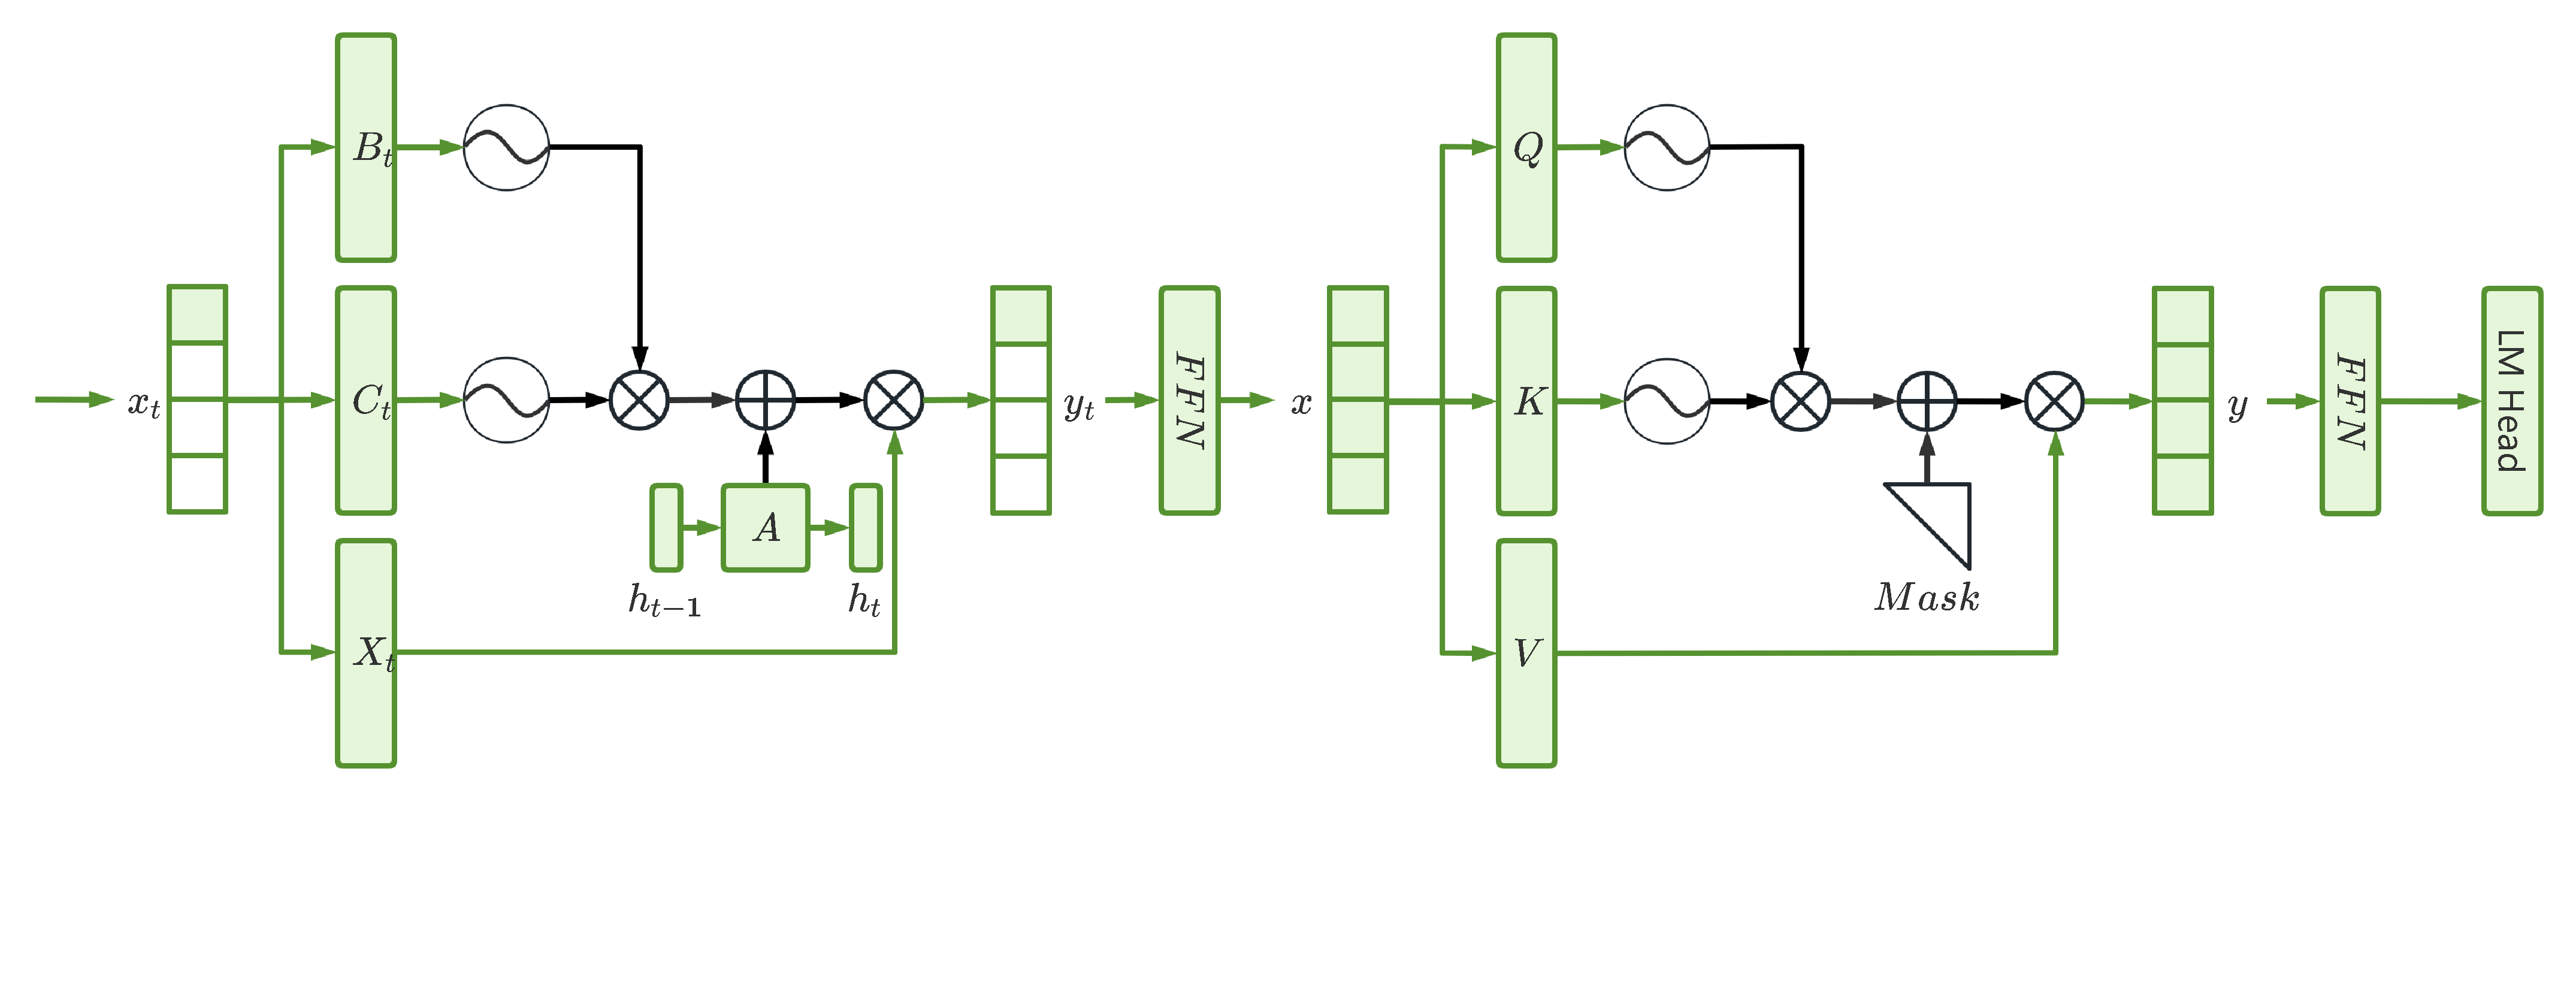
\includegraphics[width=\linewidth]{fig/architecture.pdf}
   \caption{
      % 状态空间和自注意力都使用相同的位置编码, 并且在 LM-Head 之前使用自注意力和前馈网络构成的 Transformer 块, 无论模型骨干的其他部分如何组合.
     \textbf{Self-Attention before LM-Head}.
      The state-space and self-attention both use the same positional encoding, and a Transformer block composed of self-attention and feed-forward networks is used before the LM-Head, regardless of how the other parts of the model backbone are combined.
   }
   \label{fig:architecture}
\end{figure*}


% \section{Background}
% \subsection{Selective State Space Models}


% Selective state space models~\cite{gu2023mamba} consider that a fundamental problem in sequence modeling is to compress the context into a smaller state. From this perspective, the attention mechanism of Transformers explicitly stores the entire context information, as if reviewing all previous inputs and generated tokens before writing each token. In contrast, RNNs only refer to a fixed number of previous tokens each time, which allows for faster writing but may forget key tokens.

% In the precursor state space models of selective state space models, there are 4 parameters$(\Delta t, A, B, C)$, and they do not change with the input. These parameters control the following two stages:
% \begin{align}
%    h'(t) &= Ah(t) + Bx(t) \quad \text{(1a)} \nonumber \\
%    y(t) &= Ch(t) \quad \text{(1b)} \nonumber \\
%    h_t &= \overline{A}h_{t-1} + \overline{B}x_t \quad \text{(2a)} \nonumber \\
%    y_t &= Ch_t \quad \text{(2b)} \nonumber \\
%    \overline{K} &= (C\overline{B}, C\overline{A}\overline{B}, \ldots, C\overline{A}^{k-1}\overline{B}, \ldots) \quad \text{(3a)} \nonumber \\
%    y &= x * \overline{K} \quad \text{(3b)} \nonumber
% \end{align}
% \begin{itemize}
%    \item In the first stage (1a \& 1b), the continuous parameters $h'(t)$ are transformed into discrete parameters $h_t$ through a fixed formula $\overline{A} = f_A(\Delta t, A)$ and $\overline{B} = f_B(\Delta t, A, B)$, where $(f_A, f_B)$ is called the discretization rule. The most common is the zero-order hold (ZOH) rule, defined as $\overline{A} = \exp(\Delta t A)$ and $\overline{B} = (\Delta t A)^{-1} (\exp(\Delta t A) - I) \cdot \Delta t B$.
%    \item In the second stage (2a \& 2b and 3a \& 3b), after the parameters are transformed from $(\Delta t, A, B, C)$ to $(\overline{A}, \overline{B}, C)$, linear recursion or global convolution can be used for computation.
% \end{itemize}
% State space models cannot update states selectively based on different input information.

% The solution of selective state space models (Mamba~\citep{gu2023mamba}) is that, compared to state space models that compress all historical information, they design a simple selection mechanism that parameterizes the input of the state space model,making $(\Delta t, B, C)$  a function of the input.


% \subsection{Theorems and such}
% The preferred way is to number definitions, propositions, lemmas, etc. consecutively, within sections, as shown below.
% \begin{definition}
% \label{def:inj}
% A function $f:X \to Y$ is injective if for any $x,y\in X$ different, $f(x)\ne f(y)$.
% \end{definition}
% Using \cref{def:inj} we immediate get the following result:
% \begin{proposition}
% If $f$ is injective mapping a set $X$ to another set $Y$, 
% the cardinality of $Y$ is at least as large as that of $X$
% \end{proposition}
% \begin{proof} 
% Left as an exercise to the reader. 
% \end{proof}
% \cref{lem:usefullemma} stated next will prove to be useful.
% \begin{lemma}
% \label{lem:usefullemma}
% For any $f:X \to Y$ and $g:Y\to Z$ injective functions, $f \circ g$ is injective.
% \end{lemma}
% \begin{theorem}
% \label{thm:bigtheorem}
% If $f:X\to Y$ is bijective, the cardinality of $X$ and $Y$ are the same.
% \end{theorem}
% An easy corollary of \cref{thm:bigtheorem} is the following:
% \begin{corollary}
% If $f:X\to Y$ is bijective, 
% the cardinality of $X$ is at least as large as that of $Y$.
% \end{corollary}
% \begin{assumption}
% The set $X$ is finite.
% \label{ass:xfinite}
% \end{assumption}
% \begin{remark}
% According to some, it is only the finite case (cf. \cref{ass:xfinite}) that is interesting.
% \end{remark}
% %restatable

% \subsection{Citations and References}

% Please use APA reference format regardless of your formatter
% or word processor. If you rely on the \LaTeX\/ bibliographic
% facility, use \texttt{natbib.sty} and \texttt{icml2025.bst}
% included in the style-file package to obtain this format.

% Citations within the text should include the authors' last names and
% year. If the authors' names are included in the sentence, place only
% the year in parentheses, for example when referencing Arthur Samuel's
% pioneering work \yrcite{Samuel59}. Otherwise place the entire
% reference in parentheses with the authors and year separated by a
% comma \cite{Samuel59}. List multiple references separated by
% semicolons \cite{kearns89,Samuel59,mitchell80}. Use the `et~al.'
% construct only for citations with three or more authors or after
% listing all authors to a publication in an earlier reference \cite{MachineLearningI}.

% Authors should cite their own work in the third person
% in the initial version of their paper submitted for blind review.
% Please refer to \cref{author info} for detailed instructions on how to
% cite your own papers.

% Use an unnumbered first-level section heading for the references, and use a
% hanging indent style, with the first line of the reference flush against the
% left margin and subsequent lines indented by 10 points. The references at the
% end of this document give examples for journal articles \cite{Samuel59},
% conference publications \cite{langley00}, book chapters \cite{Newell81}, books
% \cite{DudaHart2nd}, edited volumes \cite{MachineLearningI}, technical reports
% \cite{mitchell80}, and dissertations \cite{kearns89}.

% Alphabetize references by the surnames of the first authors, with
% single author entries preceding multiple author entries. Order
% references for the same authors by year of publication, with the
% earliest first. Make sure that each reference includes all relevant
% information (e.g., page numbers).

% Please put some effort into making references complete, presentable, and
% consistent, e.g. use the actual current name of authors.
% If using bibtex, please protect capital letters of names and
% abbreviations in titles, for example, use \{B\}ayesian or \{L\}ipschitz
% in your .bib file.

% \section*{Accessibility}
% Authors are kindly asked to make their submissions as accessible as possible for everyone including people with disabilities and sensory or neurological differences.
% Tips of how to achieve this and what to pay attention to will be provided on the conference website \url{http://icml.cc/}.

% \section*{Software and Data}

% If a paper is accepted, we strongly encourage the publication of software and data with the
% camera-ready version of the paper whenever appropriate. This can be
% done by including a URL in the camera-ready copy. However, \textbf{do not}
% include URLs that reveal your institution or identity in your
% submission for review. Instead, provide an anonymous URL or upload
% the material as ``Supplementary Material'' into the OpenReview reviewing
% system. Note that reviewers are not required to look at this material
% when writing their review.

% % Acknowledgements should only appear in the accepted version.
% \section*{Acknowledgements}

% \textbf{Do not} include acknowledgements in the initial version of
% the paper submitted for blind review.

% If a paper is accepted, the final camera-ready version can (and
% usually should) include acknowledgements.  Such acknowledgements
% should be placed at the end of the section, in an unnumbered section
% that does not count towards the paper page limit. Typically, this will 
% include thanks to reviewers who gave useful comments, to colleagues 
% who contributed to the ideas, and to funding agencies and corporate 
% sponsors that provided financial support.

% \section*{Impact Statement}

% Authors are \textbf{required} to include a statement of the potential 
% broader impact of their work, including its ethical aspects and future 
% societal consequences. This statement should be in an unnumbered 
% section at the end of the paper (co-located with Acknowledgements -- 
% the two may appear in either order, but both must be before References), 
% and does not count toward the paper page limit. In many cases, where 
% the ethical impacts and expected societal implications are those that 
% are well established when advancing the field of Machine Learning, 
% substantial discussion is not required, and a simple statement such 
% as the following will suffice:

% ``This paper presents work whose goal is to advance the field of 
% Machine Learning. There are many potential societal consequences 
% of our work, none which we feel must be specifically highlighted here.''

% The above statement can be used verbatim in such cases, but we 
% encourage authors to think about whether there is content which does 
% warrant further discussion, as this statement will be apparent if the 
% paper is later flagged for ethics review.


% In the unusual situation where you want a paper to appear in the
% references without citing it in the main text, use \nocite
% \nocite{langley00}

\bibliography{paper}
\bibliographystyle{icml2025}


%%%%%%%%%%%%%%%%%%%%%%%%%%%%%%%%%%%%%%%%%%%%%%%%%%%%%%%%%%%%%%%%%%%%%%%%%%%%%%%
%%%%%%%%%%%%%%%%%%%%%%%%%%%%%%%%%%%%%%%%%%%%%%%%%%%%%%%%%%%%%%%%%%%%%%%%%%%%%%%
% APPENDIX
%%%%%%%%%%%%%%%%%%%%%%%%%%%%%%%%%%%%%%%%%%%%%%%%%%%%%%%%%%%%%%%%%%%%%%%%%%%%%%%
%%%%%%%%%%%%%%%%%%%%%%%%%%%%%%%%%%%%%%%%%%%%%%%%%%%%%%%%%%%%%%%%%%%%%%%%%%%%%%%
\newpage
\appendix
\onecolumn
\section{You \emph{can} have an appendix here.}

You can have as much text here as you want. The main body must be at most $8$ pages long.
For the final version, one more page can be added.
If you want, you can use an appendix like this one.  

The $\mathtt{\backslash onecolumn}$ command above can be kept in place if you prefer a one-column appendix, or can be removed if you prefer a two-column appendix.  Apart from this possible change, the style (font size, spacing, margins, page numbering, etc.) should be kept the same as the main body.
%%%%%%%%%%%%%%%%%%%%%%%%%%%%%%%%%%%%%%%%%%%%%%%%%%%%%%%%%%%%%%%%%%%%%%%%%%%%%%%
%%%%%%%%%%%%%%%%%%%%%%%%%%%%%%%%%%%%%%%%%%%%%%%%%%%%%%%%%%%%%%%%%%%%%%%%%%%%%%%


\end{document}


% This document was modified from the file originally made available by
% Pat Langley and Andrea Danyluk for ICML-2K. This version was created
% by Iain Murray in 2018, and modified by Alexandre Bouchard in
% 2019 and 2021 and by Csaba Szepesvari, Gang Niu and Sivan Sabato in 2022.
% Modified again in 2023 and 2024 by Sivan Sabato and Jonathan Scarlett.
% Previous contributors include Dan Roy, Lise Getoor and Tobias
% Scheffer, which was slightly modified from the 2010 version by
% Thorsten Joachims & Johannes Fuernkranz, slightly modified from the
% 2009 version by Kiri Wagstaff and Sam Roweis's 2008 version, which is
% slightly modified from Prasad Tadepalli's 2007 version which is a
% lightly changed version of the previous year's version by Andrew
% Moore, which was in turn edited from those of Kristian Kersting and
% Codrina Lauth. Alex Smola contributed to the algorithmic style files.
